\maketitle
\setcounter{page}{1}
\newpage
\pagenumbering{arabic}
\section{Zielsetzung}
  Ziel des Versuchs ist die Lebensdauerbestimmung von Myonen. Diese entstehen
  in der Hochatmosphäre und erreichen aufgrund ihrer relativistischen Geschwindigkeit
  den Erdboden, was einen Nachweis mit Szintillationsdetektoren möglich macht.
\section{Theorie}
  \subsection{Elementarteilchen}
  Im Standartmodell werden zwei Arten Elementarteilchen unterschieden:
  \begin{itemize}
    \item Bosonen
    \item Fermionen.
  \end{itemize}
  Wärend erstere als Austauschteilchen der fundamentalen Wechselwirkungen fungieren,
  stellen letztere die kleinsten aktuell bekannten Bausteine der Materie da.
  Fermionen werden dabei in Quarks und Leptonen unterteilt. Quarks bilden dabei die
  fundamentalen Bausteine der Hadronen (z.B. Baryonen wie Protonen und Neutronen,
  aber auch Mesonen). Sowohl Leptonen als auch Quarks sind in drei Generationen
  zusammengefasst. Die Fermionengenerationen umfassen:
  \begin{itemize}
    \item[I] Elektron ($\symup{e}^-$) und Elektron-Neutrino ($\symup\nu_{\symup{e}}$)
    \item[II] Myon ($\symup\mu^-$) und Myon-Neutrino ($\symup\nu_{\symup\mu}$)
    \item[III] Tauon ($\symup\tau^-$) und Tauon-Neutrino ($\symup\nu_{\symup\tau}$).
  \end{itemize}
  Elektron, Myon und Tauon sind dabei 1-fach negativ geladen und Massebehaftet,
  die entsprechenden Neutrinos sind ungeladen und haben eine im Standartmodell
  verschwindende Masse.\\
  All diesen Teilchen ist ein entsprechendes Antiteilchen zugeordnet. Für die geladenen
  Teilchen wird dies mit einem hochgestellten $+$ anstelle des $-$ gekennzeichnet, die
  Antiteilchen sind 1-fach positiv geladen.
  Antineutrinos erhalten eine Überstreichung. Lediglich das Antiteilchen des Elektrons
  ist als Positron benannt. Das Elektron ist das einzige stabile geladene Lepton.
  \subsection{Kosmische Myonen}
  Myonen entstehen in vielfältigen Prozessen, beispielsweise beim Zerfall von geladenen
  Pionen:
  \begin{equation*}
    \pi^+ \to \mu^+ + \nu_{\mu} \qquad \text{ und } \qquad \pi^- \to \mu^- + \bar{\nu}_{\mu} .
  \end{equation*}
  Diese entstehen beispielsweise in der Hochatmosphäre in sogenannten ausgedehnten
  Luftshowern (EAS). Insbesondere hochrelativistische Protonen aus extraterestrischen
  Quellen (z.B. aus aktiven Galaxienkernen) können als primäre
  Partikel einen solchen EAS auslösen. Durch Wechselwirkungen mit Luftmolekülen
  entstehen unter anderem Pionen, aus deren Zerfallsprodukten Myonen frei werden.
  Diese Myonen tragen einen Teil der Energie des Primärteilchens und bewegen sich
  daher aufgrund ihrer im Vergleich zum einfallenden Proton geringen Masse ebenfalls mit
  annäherder Lichtgeschwindigkeit. Aufgrund der resultierenden Zeitdilatation
  können sie trotz ihrer geringen Lebensdauer den Erdboden erreichen.
  \subsection{Verhalten von Myonen in Szintillationsdetektoren}
  Myonen können mit einem Szintillationsdetektor nachgewiesen werden. Bei ihrem Durchgang
  durch den Szintillator deponieren sie einen Teil ihrer kinetischen Energie im Szintillatormaterial.
  Dies äußert sich in Form von Anregungszuständen der Moleküle, bei deren Rückkehr in
  den Grundzustand Photonen frei werden. Diese können durch Sekundärelektronenvervielfacher
  (SEV - aufgebaut aus einer Photokathode, Dynoden zur Sekundärelektronenproduktion sowie
  einer Anode) nachgewiesen werden.\\
  Es sind nun drei Fälle zu unterscheiden:
    \begin{enumerate}
    \item Das Myon hat auf seinem Weg durch die Atmosphäre bereits viel Energie
    verloren und zerfällt im Detektor:\\
    In diesem Fall ist eine Lebensdauerbestimmung möglich. Beim Eintritt in den Detektor
    wird nach dem oben geschilderten Prinzip ein detektierbares Signal erzeugt. Bei
    seinem Weg durch den Detektor zerfällt das Myon in ein Elektron oder Positron\footnote{
    Bei dem angegeben Zerfallskanal handelt es sich lediglich um den mit Abstand häufigsten,
    es existieren weitere.}:
    \begin{align*}
      \mu^+ &\to e^+ + \nu_{e} + \bar{\nu}_{\mu}\\
      \mu^- &\to e^- + \bar{\nu}_{e} +  \nu_{\mu}.
    \end{align*}
    Das entstehende Elektron (oder Positron) ist wiederum  aufgrund seiner hohen Energie
    in der Lage das Szintillatormaterial anzuregen.
    Durch die dabei entstehenden Photononen wird ein zweites Signal detektierbar
    und aus der Zeitdifferenz lässt sich die Lebensdauer berechnen.
    \item Das Myon durchquert den Detektor ohne zu Zerfallen:\\
    In diesem Fall wird lediglich das erste Signal detektiert, das zweite nicht.
    Dies ist schaltungstechnisch zu berücksichtigen (siehe Kapitel \ref{sec:Aufbau}).
    \item Einfang negativer Myonen durch Szintillatoratome:\\
    Analog zum Elektroneneinfang können negative Myonen mit einer gewissen Wahrscheinlichkeit
    unter Bildung eines myonischen Atoms eingefangen werden. Wie beim Durchqueren
    des Detektorn bleibt hier das zweite Signal aus.
    \end{enumerate}
  \subsection{Lebensdauer von Teilchen}
  \label{sec:Lebensdauer}
  Bei Teilchenzerfällen handelt es sich um statistische Prozesse.
  Zuerst wird die Wahrscheinlichkeit $\symup{d}W$,
  dass ein Zerfall im Zeitraum $\symup{d}t$ eintritt, betrachet.
  Unter Annahme von Proportionalität zwischen $\symup{d}W$ und $\symup{d}t$ folgt der Zusammenhang
  \begin{equation*}
    \symup{d}W = \lambda\symup{d}t,
  \end{equation*}
  $\lambda$ stellt hier eine charakteristische Konstante dar. Die Zerfallswahrscheinlichkeit
  ist offensichtlich unabhängig vom individuellen Alter eines Teilchens.
  Die Zerfälle mehrerer Teilchen sollten statistisch unabhängig von einander sein.
  Unter dieser Annahme folgt weiter:
  \begin{equation*}
    \symup{d}N = -N\symup{d}W = - \lambda N \symup{d}t,
  \end{equation*}
  dabei ist $\symup{d}N$ die Zahl der Teilchen, die im Zeitraum $\symup{d}t$ zerfallen sind, wenn
  $N$ Teilchen beobachtet werden. Für große $N$ lässt sich durch Integration das exponentielle
  Zerfallsgesetz gewinnen:
  \begin{equation}
    \frac{N(t)}{N_0} = \exp{(-\lambda t)}.
    \label{runeduhund}
  \end{equation}
  Dabei bezeichnet $\lambda$ hier die teilchenspezifische Zerfallskonstante,
  $t$ die Zeit und $N_0$ die zum Zeitpunkt $t=0$ vorhandenen Teilchen.
  In einem Intervall $[t, \symup{d}t]$ lässt sich daraus die Verteilungsfunktion
  bestimmen, der die Lebensdauern der Teilchen folgen:
  \begin{equation*}
    \symup{d}N \left( t \right) = N_0 \cdot \lambda \cdot \symup{exp} \left( - \lambda t \right) \symup{d}t \; .
  \end{equation*}
  Bestimmen des ersten Momentes dieser Verteilung leifert den Erwartungswert für die Lebensdauer:
  \begin{equation}
    <t> = \tau = \int_0^\infty \lambda t \exp{(-\lambda t)} \symup{d}t =
    \left| \lambda \left( -\frac{t}{\lambda} - \frac{1}{\lambda^2} \right)\exp{(-\lambda t)}
    \right|_0^\infty = \frac{1}{\lambda}.
    \label{eq:tau}
  \end{equation}
  \subsection{Statistische Probleme}
  Wäre es möglich, beliebig viele Lebensdauern zu messen, würde die Verteilung
  der Messwerte im Limes $N \to \infty$ gegen die im Kapitel $\ref{sec:Lebensdauer}$
  bestimmte Verteilungsfunktion \eqref{runeduhund} konvergieren. Experimentell ist jedoch immer nur
  eine Stichprobe zugänglich. Hier kommen insbesondere Punktschätzer wie das
  arithmetische Mittel infrage, um den Erwartungswert einer Stichprobe zu bestimmen.
  Wäre es grundsätzlich möglich, jeden Messwert aufzunehmen,
  würde das arithmetische Mittel auch gegen den Erwartungswert konvergieren.
  Diese Bedingung ist hier jedoch nicht erfüllt, das Intervall der theoretisch
  aufzunehmenden Messwerte wird durch den Versuchaufbau begrenzt. Es muss daher
  auf nichtlineare Ausgleichsrechnung, beispielsweise mittels der Methode der kleinsten Fehlerquadrate,
  zurückgegriffen werden. Eine gute Abschätzung für die Lebensdauer wird also durch
  Regression durch die Messwerte mit der Verteilungsfunktion gewonnen.
\section{Durchführung}
  \subsection{Versuchsaufbau}
  \label{sec:Aufbau}
  \subsubsection{Grundlegende Messmethode:}
  	Ein Blockschaltbild des Versuchsaufbaus ist in Abbildung \ref{fig:aufbau} dargestellt.
  	Der Szintillatorbehälter besteht dabei aus einem Edelstahlzylinder, an dessen
  	Enden jeweils ein SEV optisch angekoppelt ist. Das Szintillatormedium ist organisch
  	und im Edelstahltank in Toluol gelöst. Die im Szintillator angeregten Elektronen besitzen eine
  	Abklingzeit im Bereich von \SI{10}{\nano\second}.\\
  	Bestimmt werden soll nun die Zeit zwischen dem ersten (Eintritt in den
  	Detektor) und dem zweiten Lichtimpuls (Zerfall im Detektor). Dazu wird ein
  	Zeit-Amplituden-Konverter (TAC) genutzt. Der TAC gibt einen Spannungsimpuls ab,
  	dessen Höhe proportional zum zeitlichen Abstand der
  	beiden Signale ist. Zum Bestimmen der Zeitabstände wird eine Stopp-Uhr genutzt.
    Der erste Impuls startet ein Zählwerk, der zweite stoppt es.
    Der am TAC entstehende Impuls wird anschließend in einem Vielkanalanalysator
  	entsprechend seiner Höhe in einem Kanal einordnet und gespeichert.
  	Die Daten werden über einen Rechner ausgelesen.
  	\begin{figure}[p]
    	\centering
    	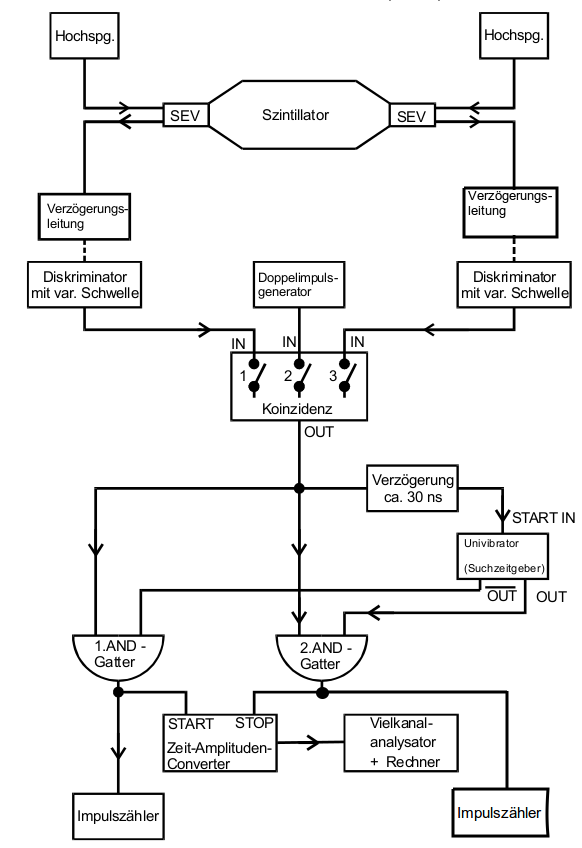
\includegraphics[width=0.7\textwidth]{Bilder/AufbauB.png}
    	\caption{Blockschaltbild des Versuchsaufbaus, verändert nach \cite{anleitung}.}
    	\label{fig:aufbau}
  	\end{figure}
  \subsubsection{Filtern von nicht-zerfallenden Myonen.}
  Die oben beschriebene Messmethode ist nicht geeignet, um die in Kapitel \ref{sec:Lebensdauer}
  beschriebenen Fälle auszuschließen, in denen das Myon nicht zerfällt, also nur
  der Eintrittslichtimpuls im Szintillator entsteht. Diese Fälle werden nun
  durch das schaltungstechnische Einbauen einer Suchzeit $T_s$ über eine monostabile
  Kippstufe (auch Univibrator) gefiltert. Die monostabile Kippstufe wird dabei durch
  den vom SEV über eine Koinzidenzschaltung (siehe Kapitel \ref{Rausch}) einlaufenden
  Impuls nach einer Verzögerung angestoßen und in einen instabilen Zustand gehoben.
  Dadurch wird das an den beiden Ausgängen des Univibrators anliegende Signal so
  getauscht, dass ein H-Signal auf das 2. AND-Gatter und ein L-Signal auf das 1. AND-Gatter
  geben wird. Nach Ablauf von $T_s$ werden die Signale wieder zurückgetauscht.
  Das Signal der Koinzidenz wird ebenfalls an das 1. und 2. AND-Gatter gegeben.\\
  Läuft nun der Einfallimpuls in die Schaltung, so liegen am 1. AND-Gatter zwei
  H-Signale (die Verzögerung vor dem Univibrator sorgt dafür, dass die Ausgänge einige
  \si{\nano\second} später umgetauscht werden). Das 1. AND-Gatter schaltet daher durch
  und den TAC erreicht das Start-Signal. Die monostabile Kippstufe schaltet nun um
  und am 2. AND-Gatter liegt ein H-Signal. Läuft in der Zeit $T_s$ nun das Zerfallssignal
  ein, liegen am 2. AND-Gatter 2 H-Signale und das Stopp-Signal für den TAC wird gegeben.
  Passiert dies nicht schaltet die Kippstufe wieder um und die Messung wird verworfen.\\
  Die Suchzeit muss so gewählt werden, dass sie groß gegenüber der Lebensdauer (Größenordnung
  \si{\micro\second}), aber klein
  gegenüber dem zeitlichen Abstand zwischen zwei einfallenden Myonen
  (Größenordnung \si{\milli\second}) ist, damit das
  Stopp-Signal nicht durch ein zweites Myon gegeben wird. Dies ist letztlich jedoch nicht
  auszuschließen und durch diese Schaltung auch nicht filterbar. Die Dauer zwischen
  zwei Myonen ist jedoch statistisch verteilt, wodurch alle Kanäle gleich stark von
  solchen Fehlmessungen betroffen sind. Es ergibt sich eine kontuierliche Untergrundrate $U$,
  die alle Kanäle gleichermaßen betrifft.
  \subsubsection{Rauschunterdrückung}
  \label{Rausch}
  Eine weitere Rauschquelle stellen spontane, thermische Elektronenemissionen der Photokathoden
  der SEVs dar. Diese führen zu Spannungssignalen, obwohl kein Myon eingefallen ist.
  Die entstehenden Signale sind jedoch meistens kleiner als die von Myonen verursachten.
  Zur Unterdrückung dieser Signale werden zwei Methoden verwendet:
  \begin{enumerate}
    \item Diskriminatoren:\\
    Beiden SEVs sind Diskriminatoren nachgeschaltet. Diese geben nur dann ein Signal
    ab, wenn das einlaufende Signal eine gewisse Schwelle überschreitet. Diese muss
    so gewählt werden, dass echte Signale möglichst nicht gefiltert werden. Die
    Diskriminatoren leisten weiterhin eine Umwandlung der einfallenden Pulse
    in eine H-Signal der NIM-Logik.
    \item Koinzidenzschaltung:\\
    Weiterhin sind gleich zwei SEVs verbaut, deren Signale über eine Koinzidenzschaltung
    abgeglichen werden. Nur wenn von beiden SEVs innerhalb einer Zeit $\symup\Delta t_K$
    ein Signal an den Eingängen der Koinzidenz ankommt, wird ein Signal weitergegeben.
    Da spontane Emissionen jeweils nur einen SEV betreffen und die Wahrscheinlichkeit,
    dass es an beiden SEVs gleichzeitig zu spontaner Emission kommt relativ gering ist,
    stellt dies eine gute Möglichkeit zur Signalfilterung dar. Die Zeit $\symup\Delta t_K$
    ist durch Variation der Diskriminatorlänge jedoch so zu wählen, dass Sie sowohl den Lichtweg zwischen den beiden SEVs
    (ca. \SI{4}{\nano\second} für den Fall, dass ein Signal unmittelbar an einem SEV
    entsteht), als auch Unterschiede in den Kabellängen der beiden Leitungen der
    SEVs zur Koinzidenz berücksichtigt. Letztere können durch eine Verzögerungsschaltung
    aufeinander abgeglichen werden.
  \end{enumerate}
  Auch durch diese beiden Möglichkeiten ist eine totale Rauschunterdrückung nicht möglich.
  \subsection{Versuchsdurchführung}
  \label{sec:Durchführung}
  \subsubsection{Aufbau und Justage des Versuchsaufbaus}
  Die Schaltung wird schrittweise aufgebaut und unter Zuhilfenahme eines Oszillographen
  überprüft und justiert. Es wird mit dem zur Rauschunterdrückung gedachten
  Teil des Aufbaus begonnen:
  \begin{enumerate}
    \item Nach Einschalten der Hochspannung sollen an den SEV Ausgängen Impulse
    unterschiedlicher Höhe abfallen.
    \item Die Länge der Diskriminatorpulse wird gemessen.
    \item Über ein Zählwerk wird die Zahl der pro Zeitintervall einfallenden Myonen
    gemessen. Die Diskriminatoren werden so eingeregelt, dass sie zwischen 20 und 40
    Myonen pro Sekunde liegt. An beiden Diskriminatoren sollte in etwa die gleiche
    Rate abfallen.
    \item Es wird die Koinzidenzschaltung angeschlossen und der Ausgang auf ein
    Zählwerk gelegt. Die Zählrate wird abhängig von der Verzögerung gemessen, am
    entsprechenden Graphen sollte sich ein "Plateau" bilden. Bei der zum Maximum
    korespondierenden Verzögerung wird die Messung durchgeführt, aus der Halbwertsbreite
    der Kurve lässt sich später die Verzögerungszeit rekonstruieren.
    \item Zuletzt wird die Zählrate vor und hinter der Koinzidenz verglichen. Sollte
    diese annähernd gleich sein, muss die Diskriminatorschwelle gesenkt werden um die
    Myonenrate zu erhöhen. Ansonsten ist die Koinzidenz wirkungslos.
  \end{enumerate}
  Zum weitern Aufbau wird der Teil vor der Koinzidenzschaltung abgeklemmt und ein
  Doppelimpulsgenerator auf den an der Koinzidenz verbleibenden Eingang gelegt.
  Die Dauer zwischen zwei von Doppelimpulsgenerator gegebenen Inpulsen ist einstellbar
  und lässt sich gut zum Überprüfen der Schaltung nutzen.
  \begin{enumerate}
    \item Der Univibrator wird über die Verzögerungsleitung angeschlossen. An den
    Ausgängen der Kippstufe kann nun die Suchzeit gemessen werden. Diese sollte den
    Zeitmessbereich des TAC nur leicht überschreiten.
    \item Die AND-Gatter werden entsprechend des Blockschaltplans eingebaut. Die von
    den AND-Gattern auf die Eingänge des TAC gehenden Signale müssen den selben Abstand
    haben, der zwischen den Impulsen am Doppelimpulsgenerator eingestllt ist.
    \item Der TAC wird überprüft. Die Höhe der am Ausgang abfallenden Signale muss
    dabei proportional zum eingestellten Impulsabstand sein.
    \item Abschließend wird durch Variation der Impulsabstände überprüft, welcher Kanal
    am Vielkanalanalysator welcher Messzeit entspricht.
  \end{enumerate}
  \subsubsection{Messung}
  Die Messung wird begonnen, indem Zählwerk und Vielkanalanalysator gleichzeitig
  gestartet werden. Die Messzeit beträgt zwischen 20 und \SI{30}{\hour}.
  Zum Beenden der Messung werden Zählwerk und Vielkanalanalysator gleichzeitig gestoppt.
  Aufgezeichnet werden die Ergebnisse des Vielkanalanalysators, die Anazahl der detektierten
  Myonen, die Anzahl der Fehlmessungen sowie der Messzeit.

\section{Auswertung}

\subsection{Fehlerrechnung}
  Für die Auswertung wird als Punktschätzer der arithmetischen Mittelwert
  \begin{equation}
    \overline{T}_{\symup{arith.}} = \frac{1}{n} \sum_{i=1}^{n} T_{i}
    \label{arith}
  \end{equation}
  genutzt.
    Für die Fehlerrechnung sowie den mathematischen Teil der Auswertung wird auf $\textsc{Python}$ \cite{python}
    zurückgegriffen:\\
    Arithmetische Mittelwerte werden durch die Funktion $\textsc{mean}$ aus dem Paket $\textsc{Numpy}$ \cite{numpy}
    nach \eqref{arith},
    gewichtete Mittelwerte durch manuelles implementieren der jeweiligen Funktion berechnet.
    Fehlerfortpflanzung wird
    durch die Bibliothek $\textsc{uncertainties}$ \cite{uncertainties} automatisiert.
    Regressionen sowie deren Fehler wurden durch die $\textsc{Numpy}$ Funktion $\textsc{curve-fit}$
    durchgeführt.
    Grafiken wurden mit $\textsc{matplotlib}$ \cite{matplotlib}
    erstellt.
\subsection{Bestimmung der Verzögerungszeit}
Um die Verzögerungszeit $T_{\symup{VZ}}$ zu bestimmen, wurde an einer Verzögerungsleitung eine
feste Verzögerung von \SI{20}{\nano\second} eingestellt und die Verzögerung der anderen
Verzögerungslinie von 0 bis \SI{34}{\nano\second} variiert und das jeweilige $N(t)$ bestimmt.
In Abbildung \ref{fig:1} Tabelle \ref{sub:tab1} befinden sich die Messwerte und in Abbildung \ref{sub:fig1}
die zugehörige grafische Darstellung. Die Fehler sind nach $\sqrt{N}$ gebildet worden,
also dem Poisson-Fehler für Zählexperimente.
\begin{figure}
  \centering
  \subcaptionbox{Verzögerung der zweiten Verzögerungslinie und zugehörige Zählrate. \label{sub:tab1}}[0.3\textwidth]{
  \centering
  \begin{tabular}{c c}
    \toprule
    d$t$ / \si{\nano\second} & $N$ \si{\per10\second} \\
    \midrule
    -20 & 148 \\
    -19 & 170 \\
    -18 & 193 \\
    -17 & 216 \\
    -16 & 214 \\
    -14 & 209 \\
    -12 & 213 \\
    -10 & 223 \\
    -8 & 221 \\
    -6 & 233 \\
    -4 & 246 \\
    -2 & 231 \\
    0 & 227 \\
    2 & 227 \\
    4 & 229 \\
    6 & 225 \\
    7 & 207 \\
    8 & 186 \\
    9 & 185 \\
    10 & 182 \\
    12 & 135 \\
    14 & 141 \\
    \bottomrule
  \end{tabular}
  }
  \subcaptionbox{Grafische Darstellung. Die Daten wurden um \SI{20}{\nano\second}
  zentriert. \label{sub:fig1}}[0.6\textwidth]{
  \centering
  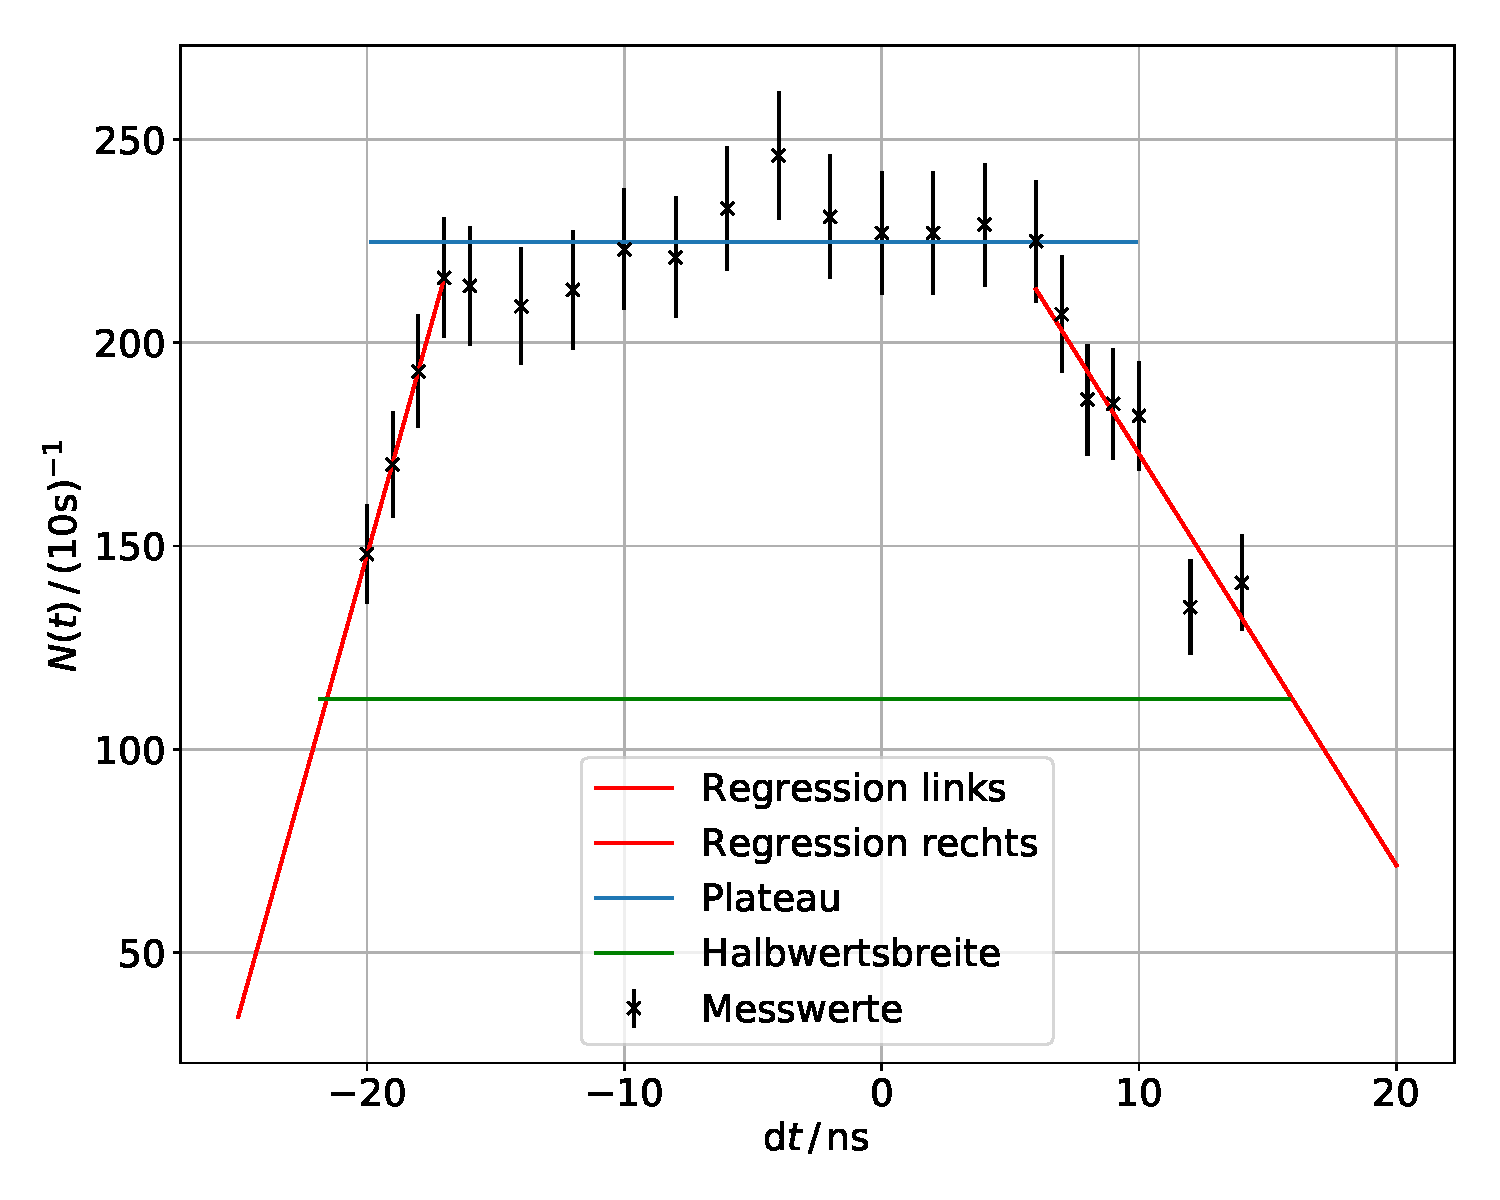
\includegraphics[width=0.6\textwidth]{Plateau.pdf}
  }
  \caption{Tabelle mit Messwerten und zugehörige grafische Darstellung.}
  \label{fig:1}
\end{figure}
Aus der Grafik \ref{sub:fig1} wird ersichtlich, dass das Maximum bei \SI{16}{\nano\second}
liegt, also insgesamt eine Verzögerung von \SI{4}{\nano\second} angelegt wurde.
Außerdem ist in Abbildung \ref{sub:fig1} die Halbwertsbreite eingetragen.
Diese ist
gleichbedeutend mit der Auflösungszeit $ \symup{\Delta}t_K$ der Koinzidenzeinheit.
Zu ihrer Bestimmung
wurde das Plateau und die Flanken jeweils mit einer linearen Funktion gefittet. Die
halbe Höhe des Plateus wird daraufhin mit den beiden Fits der Flanken geschnitten
und der Abstand der x-Werte der Schnittpunkte bestimmt.
Es folgt
\begin{equation}
  \symup{\Delta}t_K = |-22| + |16| = \SI{38}{\nano\second} \, .
\end{equation}
Die Breite der Diskriminatoren wurde zu \SI{50}{\nano\second} bestimmt. Hier zeigt
sich eine Abweichung von 24\%.

\subsection{Kalibrierung der Kanäle}
\label{sec:kal}
Um die Kanäle zu kalibrieren, wird ein Doppelimpuls mit verschieden langen Impulsabständen
durch den Messaufbau geschickt und vom Vielkanalanalysator verarbeitet. Aus eben jenen
Impulsabständen $t_{\symup{kal}}$ und der Auswertung des Vielkanalanalysators lässt sich bestimmen, welcher
Kanal mit welchem Impulsabstand korrespondiert. Da sich diese proportional zueinander
verhalten, wird eine lineare Regression mit den Messwerten in Tabelle \ref{sub:tab2}
durchgeführt. Dabei wurden von den doppelt und dreifach gefüllten Kanälen der
Kanal mit den meisten Ereignissen verwendet. Die Anzahl der Hits in den
einzelnen Kanälen insgesamt ist ebenfalls in Abbildung \ref{fig:2} Tabelle
\ref{sub:tab1} dargestellt. Aus einer Frequenz von \SI{1}{\kilo\hertz} und
einer Messdauern von \SI{10}{\second} ergeben sich sich 10000 Ereignisse.
Diese Anzahl findet sich in guter Näherung in der Tabelle wieder.
Die lineare Regression
\begin{equation*}
  f(x) = mx + b
\end{equation*}
ist in Abbildung \ref{sub:fig2}.
\begin{figure}
  \centering
  \subcaptionbox{Impulsabstände, korrespondierender Kanal und
  Anzahl der Ereignisse. \label{sub:tab2}}[0.4\textwidth]{
  \centering
  \begin{tabular}{c c c}
    \toprule
    $t_{\symup{kal}}$ / \si{\micro\second} & Kanal & \# Ereignisse \\
    \midrule
    1 & 23 & 10192 \\
    2 & 45 & 10016 \\
    3 & 67 & 10438 \\
    4 & 90 & 10338 \\
    5 & 112 & 10274 \\
    6 & 134 & 10232 \\
    7 & 156 & 10384 \\
    8 & 178 & 10422 \\
    9 & 200 & 10304 \\
    \bottomrule
  \end{tabular}
  }
  \subcaptionbox{Grafische Darstellung mit linearer Regression. \label{sub:fig2}}[0.59\textwidth]{
  \centering
  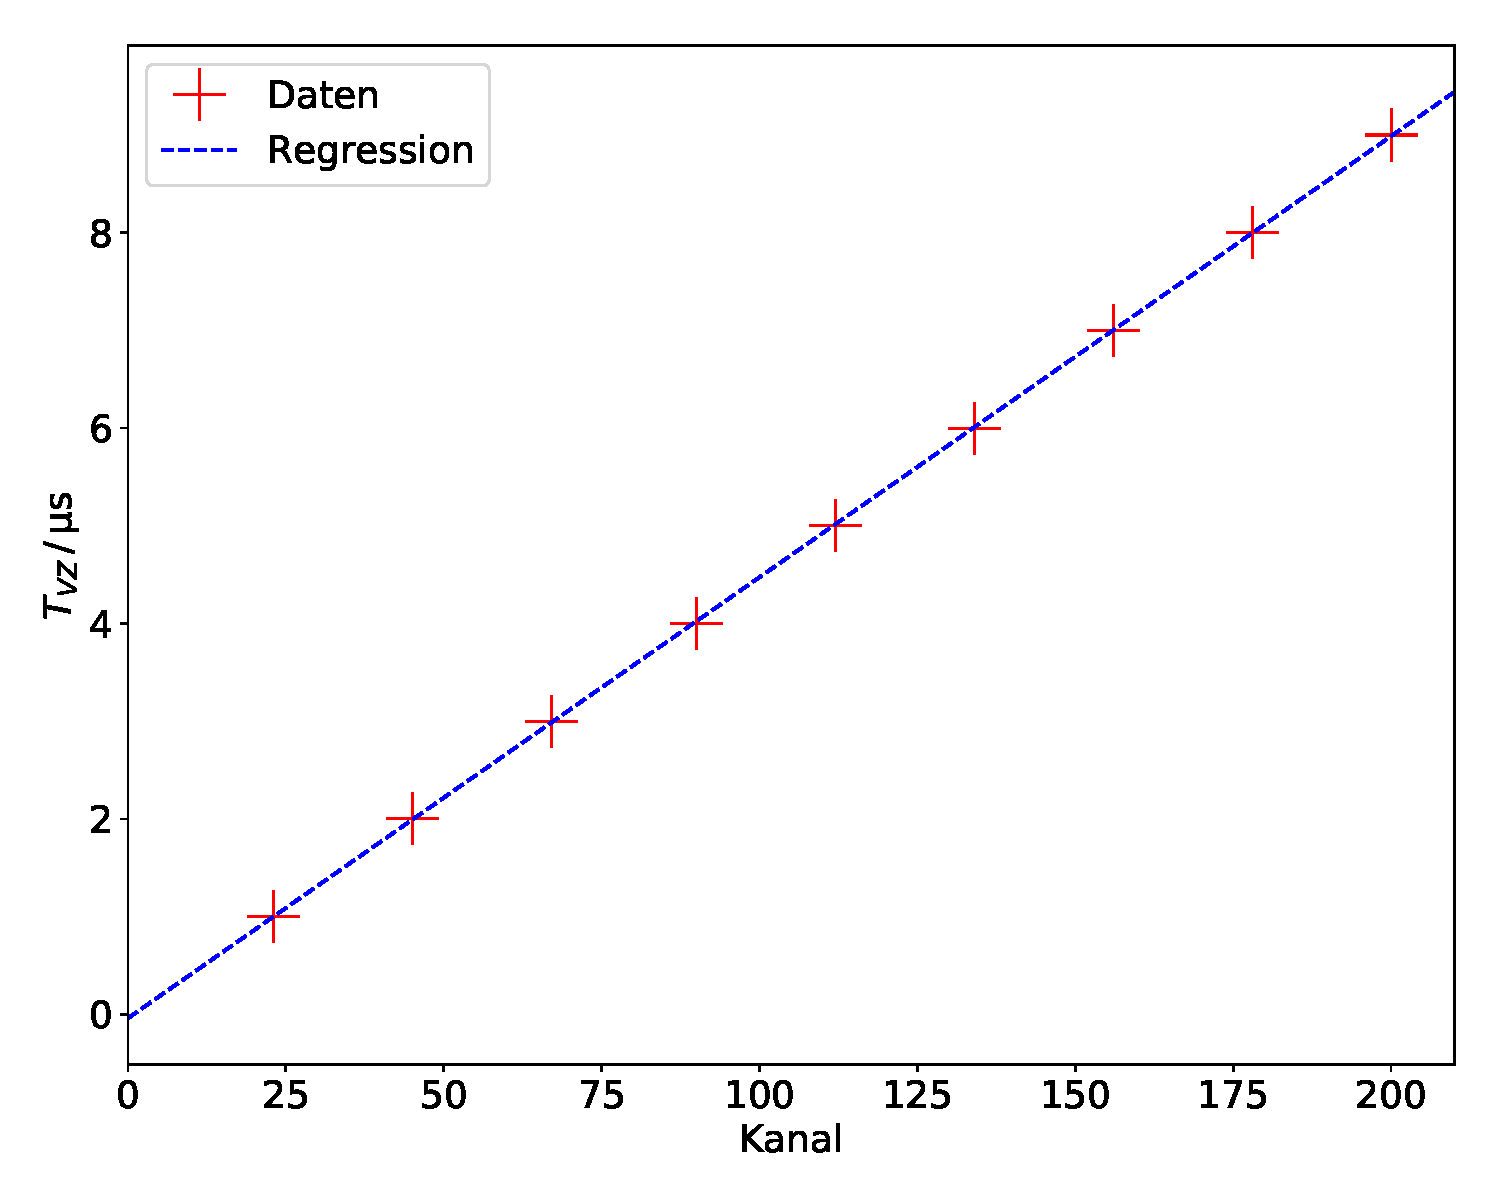
\includegraphics[width=0.59\textwidth]{kal.pdf}
  }
  \caption{Tabelle mit Messwerten und zugehörige grafische Darstellung.}
  \label{fig:2}
\end{figure}
Sie
liefert die Parameter
\begin{align}
  m &= \num{0,04515(8)} \\
  b &= \SI{-0,041(10)}{\micro\second} \, .
\end{align}
Also lassen sich die zu den einzelnen Kanälen gehörenden Zeitdauern aus einer linearen
Funktion mit den errechneten Parametern bestimmen. Dazu wurde angenommen, dass sich
auch die Kanäle > 200 linear mit den errechneten Parametern verhalten.
\subsection{Bestimmung des Untergrundes}
Zunächst gilt es, eine Ausdruck für die Anzahl der Myonen zu gewinnen, die im Mittel
den Tank durchqueren. Dieser ergibt sich aus der Anzahl
der Startimpulse und der gesamten Messzeit zu
\begin{equation}
  \overline{N} = \frac{N_{\symup{start}}}{T_{\symup{gesamt}}} \, .
\end{equation}
Während der Suchzeit $T_S$ tun dies im Mittel $n = \overline{N} \cdot T_S$ Myonen.
Die Wahrscheinlichkeit, dass dies genau $n$ Teilchen während der Suchzeit $T_S$ tun, ist
poissonverteilt. Möchte man die Fehlmessungen $N_{\symup{fehl}}$ erhalten, so muss man genau die Fälle
einbeziehen, in denen während der Suchzeit zwei Myonen direkt aufeinander gefolgt sind,
also die Anzahl aller Startimpulse mit der zugehörigen Wahrscheinlichkeit, die man
aus der Poissonverteilung erhält, multiplizieren.
Mit $N_{\symup{start}} = \num{3.0619(17)e6}$, $T_S = \SI{20}{\micro\second}$ und $T_{\symup{gesamt}}
= \SI{147182}{\second}$ folgt
\begin{equation}
  N_{\symup{fehl}} = \overline{N} \cdot T_S \cdot \symup e^{- \overline{N} \cdot T_S}
  \cdot N_{\symup{start}} = \num{1273.4(15)} \, .
\end{equation}
Der Fehler von $N_{\symup{start}}$ bestimmt sich dabei ebenfalls als Poisson-Fehler.
Da diese Ereignisse statistisch unabhängig voneinander sind, lässt sich die Untergrundrate
bestimmen aus
\begin{equation}
  U = \frac{N_{\symup{fehl}}}{\text{Anzahl Kanäle}} = \num{2.8298(32)} \, .
\end{equation}
mit 450 Kanälen.
\subsection{Bestimmung der Lebendsdauer}
Um die Lebensdauer zu bestimmen, werden als erstes die benutzten Kanäle in Zeitdauern
umgerechnet, mit der linearen Regression aus Kapitel \ref{sec:kal}. Die gemessenen
Ereignisse werden dann in Abhängigkeit der bestimmten Zeitdauern
durch eine Funktion der Gestalt
\begin{equation}
  f(t) = N_0 \cdot \symup e^{-\lambda \, t} + U_{\symup{fit}} \, ,
  \label{fit}
\end{equation}
welche im Wesentlichen \eqref{runeduhund} plus der Untergrundrate entspricht,
mit \textsc{curve-fit} gefittet. Dabei wurde $(N)^{-1/2}$ als Gewichtung
genutzt, sodass die Werte mit viel Statistik (durch einen aussagekräftigeren, weil
mit mehr Werten unterlegten Fehler) stärker gewichtet werden als Werte mit niedrigem
$N(t)$. Es wurden insgesamt 62 Werte aus der Regression rausgenommen,
da diese keine Informationen (leere Kanäle oder auußerhalb der Suchzeit) bzw. Fehlmessungen enthalten. Diese
sind im Plot markiert oder weggelassen worden, wenns sie auußerhalb der Suchzeit liegen.
Die Messwerte und die Regression mit \eqref{fit} sind in
Abbildung \ref{fig:3} zu sehen.

\begin{figure}
  \centering
  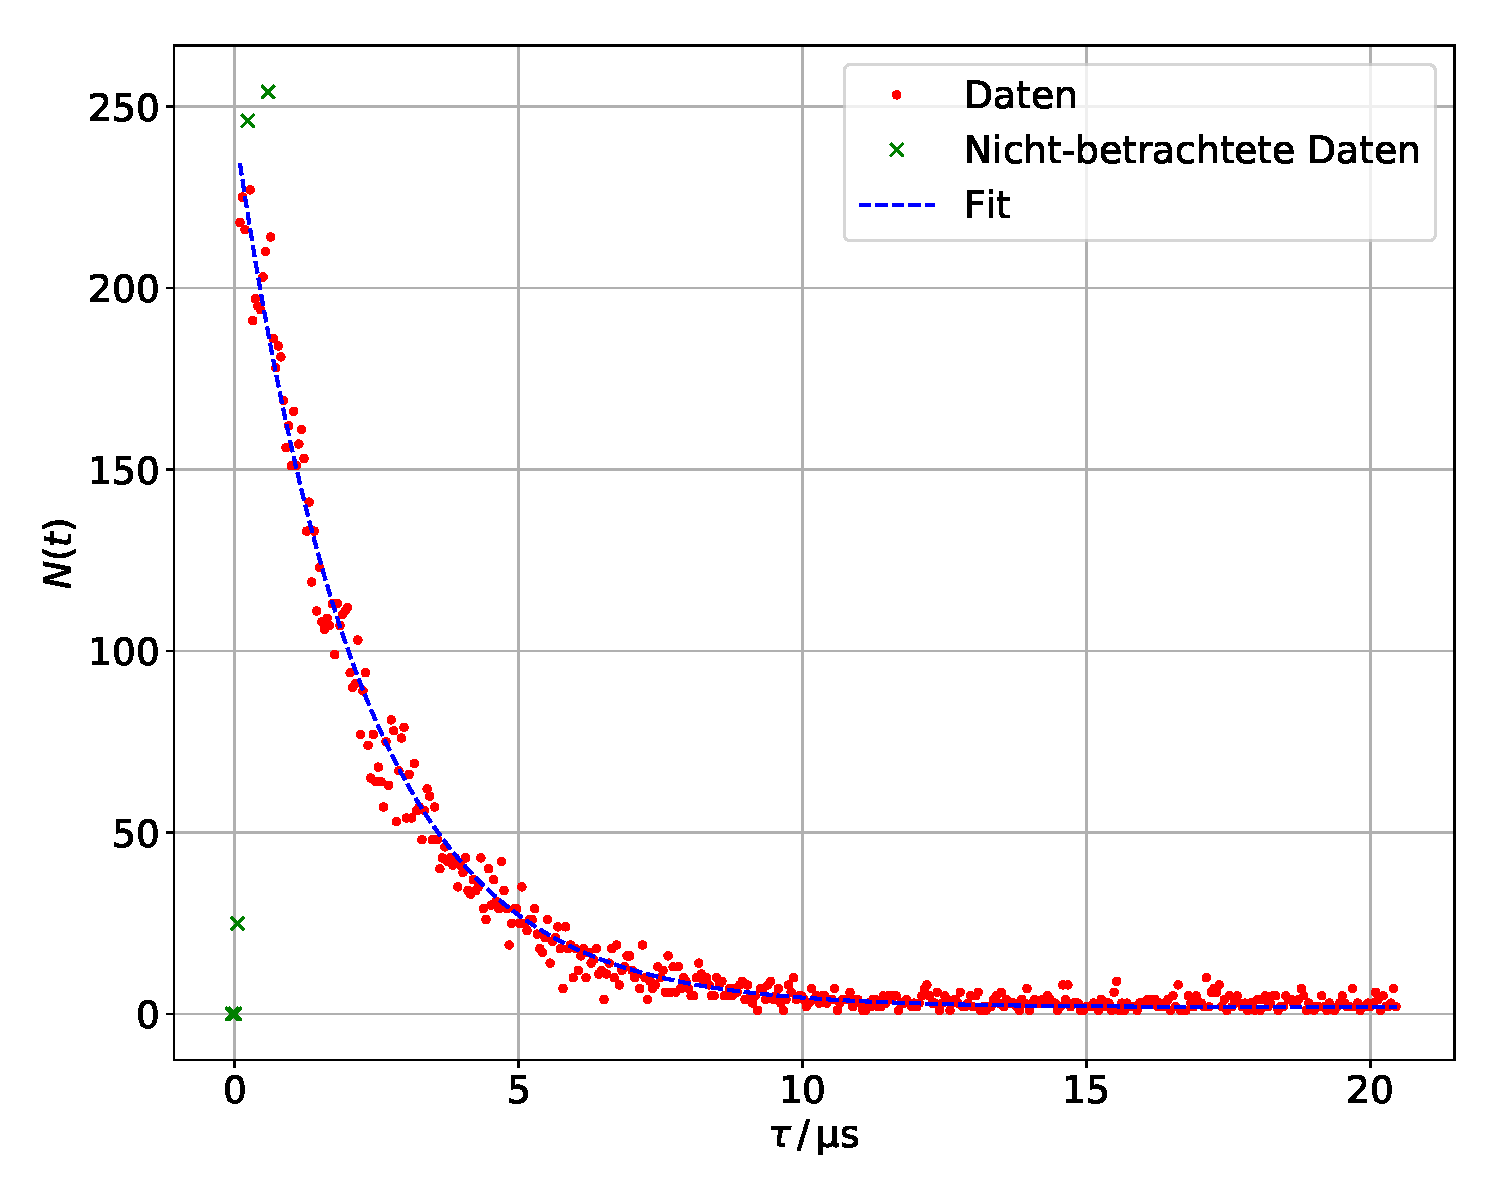
\includegraphics[scale=0.5]{fit.pdf}
  \caption{Fit mit einer Exponentialfunktion. Aus Gründe der Übersichtlichkeit
  wurde auf Fehlerbalken verzichtet.}
  \label{fig:3}
\end{figure}
Es ergeben sich für die Parameter
\begin{align}
  N_0 &= \num{242.5(16)} \ \text{pro Kanal} \\
  \lambda &= \SI{0.451(8)}{\per\micro\second} \label{dauer} \\
  U_{\symup{fit}} &= \num{1.8(13)} \ \text{pro Kanal} \label{Untergrund} \, .
\end{align}
Aus \eqref{eq:tau} ergibt sich für die Lebensdauer
\begin{equation}
  \tau = \SI{2.22(4)}{\micro\second} \, .
\end{equation}

\section{Diskusion}
\begin{table}
  \centering
  \caption{Errechnete und gefittete Werte für die Lebensdauer und die Untergrundrate.}
  \label{tab:dis}
  \begin{tabular}{c c c}
    \toprule
     &Wert aus Fit & Wert aus Literatur / Berechnung \\
    \midrule
    $\tau$ & \SI{2.22(4)}{\micro\second} & \SI{2.197}{\micro\second} \cite{lebensdauer} \\
    $U$ & \num{1.8(13)} \ \text{pro Kanal} & \num{2.8298(32)} \ \text{pro Kanal} \\
    \bottomrule
  \end{tabular}
\end{table}
Es wird ersichtlich, dass die Untergrundraten voneinander abweichen, aber der theoretisch
bestimmte Wert liegt innerhalb der Messungenauigkeit, der Fehler liegt jedoch
in der gleichen Größenordnung wie der Wert. Dies liegt an den
statistischen Schwankungen bei den hohen Lebensdauern. \\
\\
Der Literaturwert für die Lebensdauer liegt ebenfalls in der Toleranz der
errechneten Lebensdauer.
Diese gute Übereinstimmung
ließ schon Abbildung \ref{fit} vermuten, da der Fit mit der Exponential-Funktion
der Verteilung der gemessen Werten folgt. Zu den nicht-betrachteten Werten lässt sich
sagen, dass die ersten zwei Zeitdauern wohl zu klein waren, um erfasst zu werden.
Die beiden viel zu hohen Werte sind vermutlich aus der Binaddition entstanden, da
der Vielkanalanalysator auch oftmals Ereignisse auf mehrere direkt nebeneinander
liegende Kanäle verteilt. Dies ist auch schon in der Kalibrierung aufgetreten. Alles in allem ist wohl auch die hohe Anzahl an Ereignissen
für gute statistische Werte und verhältnismäßig kleine Fehler verantwortlich. Mögliche
Fehlerquellen sind die etwas ungenaue, weil von Hand eingestellte, Breite der
Diskriminatoren und die Tatsache, dass mögliche Signale durch die Maßnahmen zur
Rauschunterdrückung herausgefiltert wurden bzw. Fehlmessungen nicht herausgefiltert wurden.
Eine Anpassung würde die Kurve in Abbildung \ref{fit} in y-Richtung verschieben.
Außerdem weicht die Auflösungszeit $\symup \Delta t_K$
stark ab von den erwarteten \SI{50}{\nano\second}. Dies lässt sich durch die fehlenden
Messwerte auf den Flanken erklären, die für einen genaueren linearen Fit sorgen würden.
Vor allem auf der rechten Seite entsprechen die Messwerte nur bedingt einem linearen
Verlauf, eine genauere Messung mit mehr Messwerten würde hier weiterhelfen. \\
\\
Die Summe aller Ereignisse aus dem Vielkanalanalysator beträgt \num{1.25(18)e4} mit
einem Poissonfehler, die
am Zählwerk \num{13103}. Die Anzahl am Zählwerk liegt in der Fehlertoleranz der
Summe aus dem Vielkanalanalysator.

\newpage
\nocite{*}
\printbibliography
